% Created 2021-03-13 Sat 22:57
% Intended LaTeX compiler: xelatex
\documentclass[spanish, presentation, aspectratio=169]{beamer}
\usepackage{graphicx}
\usepackage{grffile}
\usepackage{longtable}
\usepackage{wrapfig}
\usepackage{rotating}
\usepackage[normalem]{ulem}
\usepackage{amsmath}
\usepackage{textcomp}
\usepackage{amssymb}
\usepackage{capt-of}
\usepackage{hyperref}
\usepackage{newtxsf}
\usepackage{multido}
\usepackage{tikz}
\usetikzlibrary{calc}
\usetikzlibrary{3d}
\newcommand{\setxyz}[1]{%
\pgfmathsetmacro{\xone}{cos(180+#1)}%
\pgfmathsetmacro{\yone}{sin(180+#1)}%
\pgfmathsetmacro{\xtwo}{cos(360-#1)}%
\pgfmathsetmacro{\ytwo}{sin(360-#1)}%
}
\usepackage{tikz-cd}
\usepackage{tkz-berge}
\usepackage{tkz-berge-add}
\usepackage{ytableau}
\usetikzlibrary{graphs,graphs.standard}
\usepackage[spanish, mexico, es-noshorthands]{babel}
% remove space between margin and lists
\usepackage{enumitem}
\setitemize{label=\usebeamerfont*{itemize item}%
\usebeamercolor[fg]{itemize item}
\usebeamertemplate{itemize item}}
\setlist{leftmargin=*,labelindent=0cm}
\setenumerate[1]{%
label=\protect\usebeamerfont{enumerate item}%
\protect\usebeamercolor[fg]{enumerate item}%
\insertenumlabel.}
\newcommand{\linea}[3]{%
\coordinate (Z) at ($ (#1.center)!#3!(#2.center) $);
\draw[color=green!40!black,line width=2pt]
(#1.center) -- (Z.center);}
\newcommand{\colortriang}{teal}
\newcommand{\triang}[4]{%
\shadedraw[inner color=\colortriang,opacity=#4,line width=1pt]
(#1.center) -- (#2.center) -- (#3.center) -- cycle;}
\newcommand{\trapecio}[5]{%
\coordinate (X) at ($ (#1.center)!#5!(#2.center) $);
\coordinate (Y) at ($ (#1.center)!#5!(#3.center) $);
\shadedraw[color=green!40!black,opacity=#4,line width=2pt]
(X.center) -- (Y.center) -- (#3.center) -- (#2.center) -- cycle;}
\newcommand{\suspension}[5]{%
\begin{center}%
\begin{tikzpicture}%
[scale=#2]
\setxyzvec[#3]
\begin{scope}[xyplane=-2.5]
\Vertex{x}
\end{scope}
\begin{scope}[xyplane=0]
\grEmptyCycle[RA=#4,prefix=a,rotation=#5]{#1}
\end{scope}
\EdgeFromOneToAll{x}{a}{}{#1}
\begin{scope}[xyplane=0]
\grCycle[RA=#4,prefix=a,rotation=#5]{#1}
\end{scope}
\begin{scope}[xyplane=2.5]
\Vertex{y}
\end{scope}
\EdgeFromOneToAll{y}{a}{}{#1}
\only<2->{%
\triang{a0}{a1}{y}{0.6}}
\only<3->{%
\triang{a1}{a2}{y}{0.6}}
\only<4->{%
\triang{a2}{a3}{y}{0.6}}
\only<5->{%
\triang{a3}{a4}{y}{0.6}}
\only<6->{%
\triang{a4}{a0}{y}{0.6}}
\only<7->{%
\triang{a0}{a1}{x}{0.6}}
\only<8->{%
\triang{a1}{a2}{x}{0.6}}
\only<9->{%
\triang{a2}{a3}{x}{0.6}}
\only<10->{%
\triang{a3}{a4}{x}{0.6}}
\only<11->{%
\triang{a4}{a0}{x}{0.6}}
% \begin{scope}[xyplane=-3.5]
%   \draw (0,0) node [fill=orange!80!white]{$G=\Susp C_{#1}$};
% \end{scope}
\end{tikzpicture}
\end{center}
}
\usepackage{fontawesome}
\usetheme[section page=none, numbering=none, block=fill]{metropolis}
\author{Rafael Villarroel Flores, UAEH}
\date{14 de marzo de 2021\\[0.6em] \bfseries XXXVI Coloquio Víctor Neumann-Lara}
\title{Aplicaciones de la topología combinatoria}
\beamerdefaultoverlayspecification{<+->}
\languagepath{spanish}
\hypersetup{
 pdfauthor={Rafael Villarroel Flores, UAEH},
 pdftitle={Aplicaciones de la topología combinatoria},
 pdfkeywords={},
 pdfsubject={},
 pdfcreator={Emacs 27.1 (Org mode 9.4.4)}, 
 pdflang={Spanish}}
\begin{document}

\maketitle
\setbeamercolor{alerted text}{fg=teal}

\section{Complejos simpliciales}
\label{sec:org0a75969}

\begin{frame}[label={sec:org301b3be},plain]{Parte}
\setbeamertemplate{navigation symbols}{}
\begin{tikzpicture}[remember picture,overlay]
    \node[xshift=0cm,yshift=0cm] at (current page.center) {
        
\includegraphics[width=\paperwidth]{images/paperwork}
    };
\end{tikzpicture}

\renewcommand*\sfdefault{ugq}
\sffamily\bfseries
\begin{tikzpicture}[remember picture,overlay,huge/.style={font=\Huge, inner sep=.3cm}]
  \node[%
  huge,
  right,
  align=left,
  rotate=5,
  yshift=-1cm,
  opacity=0.85,
  text width=4.4cm,
  minimum height=8.5cm,
  fill=white]%
  {\color{red!80!black}Teoría};
\end{tikzpicture}
\end{frame}

\begin{frame}[label={sec:org16cb05b}]{Complejos simpliciales}
Los complejos simpliciales proporcionan una forma inmediata de
aplicar topología en combinatoria.

\pause

\begin{definition}[Complejo simplicial]
Un \alert{complejo simplicial} \(\Delta\) es un conjunto de subconjuntos finitos de un conjunto \(X\), cerrado bajo inclusión. Los elementos de \(\Delta\) se llaman \alert{simplejos} o \alert{caras}.
\end{definition}

\begin{block}{Dimensión}
Si \(\sigma\in\Delta\) tiene \(n+1\) elementos, se dice que su
\alert{dimensión} es \(\dim\sigma=n\).

Los simplejos de dimensión \(n\) se llaman \(n\)-simplejos, los \(0\)-simplejos se llaman \alert{vértices}.
\end{block}
\end{frame}

\begin{frame}[label={sec:org75ea9ce}]{Ejemplos}
Consideremos los complejos \(\Delta_{1}\) y \(\Delta_{2}\) dados por:
\begin{align*}
\Delta_{1} &=\{\emptyset, \{1\},\{2\},\{3\},\{1,2\},\{1,3\},\{2,3\}\},\\
\Delta_{2} &=\Delta_{1}\cup\{\{1,2,3\}\}.
\end{align*}

\begin{columns}
\begin{column}{0.4\columnwidth}
\begin{figure}[htbp]
\centering
\input{complejo-01.tikz}
\end{figure}
\end{column}

\begin{column}{0.4\columnwidth}
\begin{figure}[htbp]
\centering
\input{complejo-02.tikz}
\end{figure}
\end{column}
\end{columns}
\end{frame}

\begin{frame}[label={sec:org0e6219b}]{Otro ejemplo}
Consideremos el complejo simplicial con caras maximales \(\{1,2,3,4\},\{4,5,6\},\{3,7\}\)

\begin{figure}[htbp]
\centering
\input{ejemplo-complejo.tikz}
\end{figure}
\end{frame}

\begin{frame}[label={sec:org7656403}]{Espacio topológico asociado}
\begin{itemize}
\item En general, a cualquier complejo simplicial se le asocia un espacio
topológico, llamado su \alert{realización geométrica}.

\item La realización geométrica es un \alert{funtor} de la categoría de
complejos simpliciales a la categoría de espacios topológicos.
\end{itemize}
\end{frame}

\begin{frame}[label={sec:orgb90497d}]{Complejos simpliciales en gráficas}
\begin{itemize}
\item Un primer uso de los complejos simpliciales en combinatoria se dio
en la prueba de Lovász (1978) de la conjetura de Kneser (1953):
\begin{displaymath}
\chi(KG_{n,k})=n-2k+2
\end{displaymath}

\item Para demostrarlo, Lovász asoció a cada gráfica \(G\) su \alert{complejo de
vecindades} \(\mathcal{N}(G)\), cuyo conjunto de simplejos son los conjuntos de vértices
con un vecino común.

\begin{figure}[htbp]
\centering
\input{vecindades-01.tikz}
\end{figure}
\end{itemize}
\end{frame}

\begin{frame}[label={sec:org6012feb}]{El complejo de completas}
\begin{definition}[\(\Delta(G)\)]
Dada una gráfica simple \(G\), el complejo simplicial
\(\Delta(G)\) tiene como simplejos a las subgráficas completas de \(G\).
\end{definition}

Se usa \(\Delta(G)\) para asociarle conceptos
topológicos a las gráficas.

Por ejemplo, diremos que las gráficas
\(G_{1}\), \(G_{2}\) son homotópicas si \(\Delta(G_{1})\) es
homotópico a \(\Delta(G_{2})\).
\end{frame}

\begin{frame}[label={sec:org8096587}]{Ejemplo}
Gráficas homeomorfa a la esfera \(S^{2}\):

\SetVertexNotLabeledSmall
\suspension{5}{1}{17}{1.6}{0}
\end{frame}

\begin{frame}[label={sec:orga1dd313}]{Muchos otros complejos simpliciales en combinatoria}
\begin{columns}
\begin{column}{0.5\columnwidth}
\begin{center}
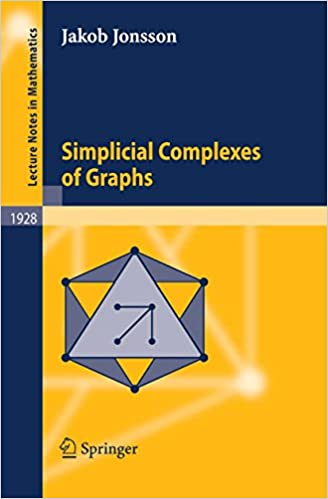
\includegraphics[height=7cm]{scog.jpg}
\end{center}
\end{column}


\begin{column}{0.5\columnwidth}
\begin{center}
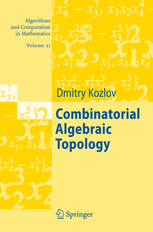
\includegraphics[height=7cm]{kozlov.jpg}
\end{center}
\end{column}
\end{columns}
\end{frame}

\begin{frame}[label={sec:org559277f}]{Topología y gráfica de clanes}
En mi investigación, me han interesado preguntas sobre la relación entre la topología y el operador de clanes. Por ejemplo:

\begin{itemize}
\item (Bandelt-Prisner, 1991, Prisner 1992) Si \(G\) es desmantelable, o si \(G\) es clan-Helly entonces \(G\simeq K(G)\).
\item \alert{Pregunta:} Si \(K^{n}(G)\) es desmantelable o clan-Helly para alguna \(n\), ¿se sigue que \(G\simeq K(G)\simeq K^{2}(G)\simeq\cdots\simeq K^{n}(G)\)?
\item (Larrión, Pizaña, V., 2013) Para toda gráfica \(H\) existe una gráfica \(G\) tal que \(G\simeq H\), con \(G\) clan-divergente.
\item \alert{Pregunta:} ¿Existe una gráfica \(G\) tal que \(G\simeq S^{2}\) y \(G\) sea clan-convergente?
\end{itemize}
\end{frame}

\section{Aplicaciones}
\label{sec:org80cc6b2}

\begin{frame}[label={sec:org7d39008},plain]{Parte}
\setbeamertemplate{navigation symbols}{}
\begin{tikzpicture}[remember picture,overlay]
    \node[xshift=0cm,yshift=0cm] at (current page.center) {
        
\includegraphics[width=\paperwidth]{images/paperwork}
    };
\end{tikzpicture}

\renewcommand*\sfdefault{ugq}
\sffamily\bfseries
\begin{tikzpicture}[remember picture,overlay,huge/.style={font=\huge, inner sep=.3cm}]
  \node[%
  huge,
  right,
  align=left,
  rotate=5,
  yshift=-1cm,
  opacity=0.85,
  text width=4.4cm,
  minimum height=8.5cm,
  fill=white]%
  {\color{red!80!black}Aplicaciones};
\end{tikzpicture}
\end{frame}

\begin{frame}[label={sec:org60948ad}]{Aplicaciones de complejos simpliciales}
Recientemente me enteré que el concepto de complejo simplicial, como \alert{generalización} del de gráfica, ha encontrado varias aplicaciones.

\begin{columns}
\begin{column}{0.3\columnwidth}
\begin{center}
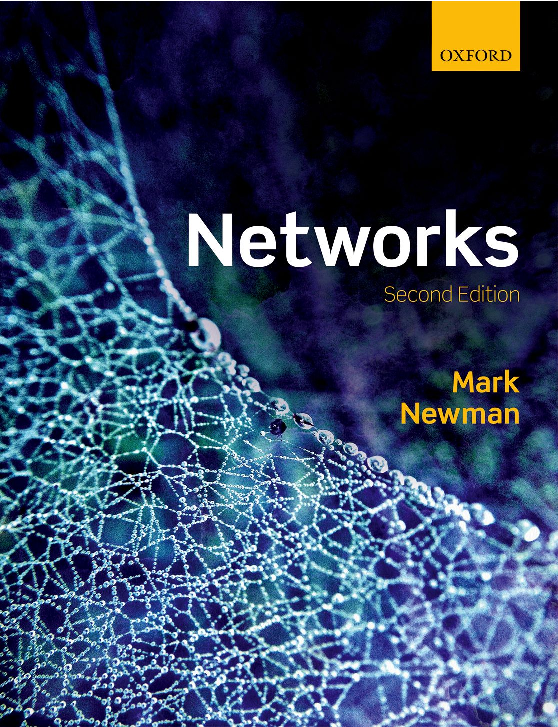
\includegraphics[height=5.2cm]{newman.pdf}
\end{center}
\end{column}

\begin{column}{0.3\columnwidth}
\begin{center}
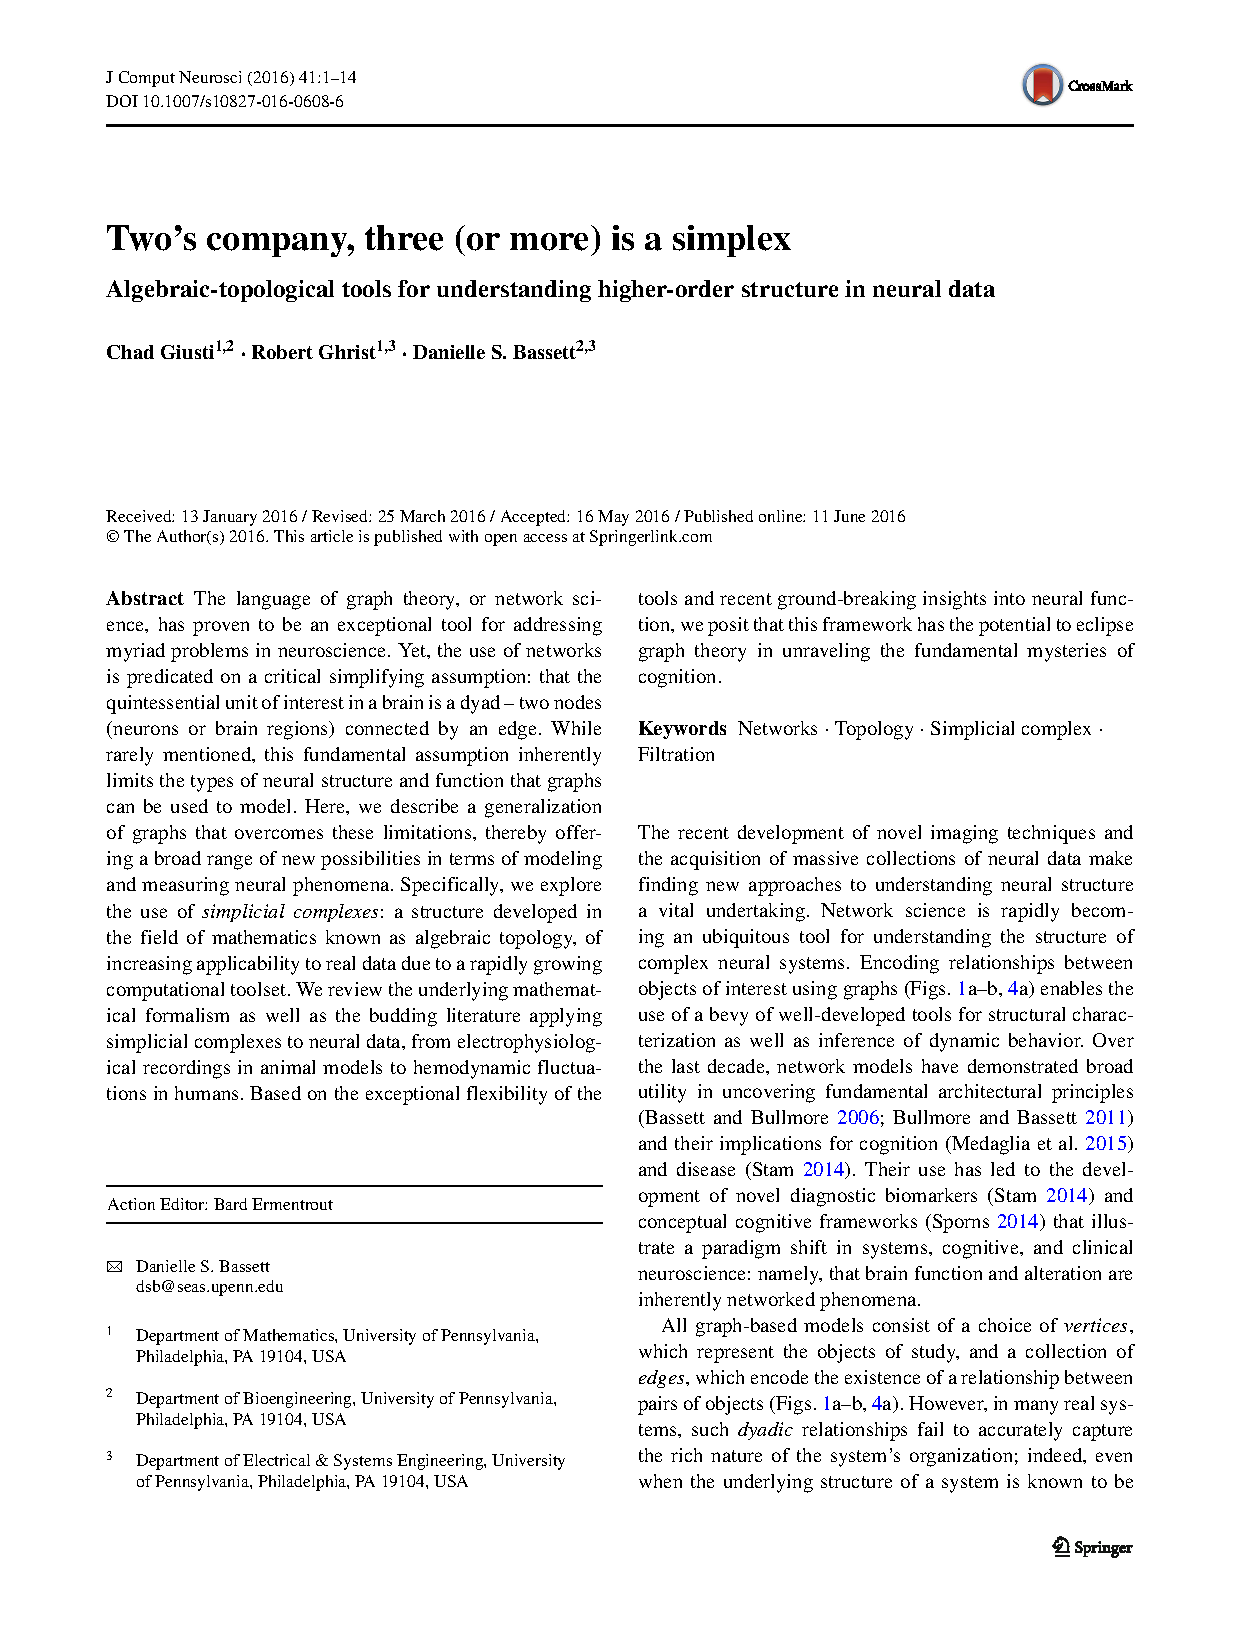
\includegraphics[height=5.2cm]{giusti1.pdf}
\end{center}
\end{column}


\begin{column}{0.3\columnwidth}
\begin{center}
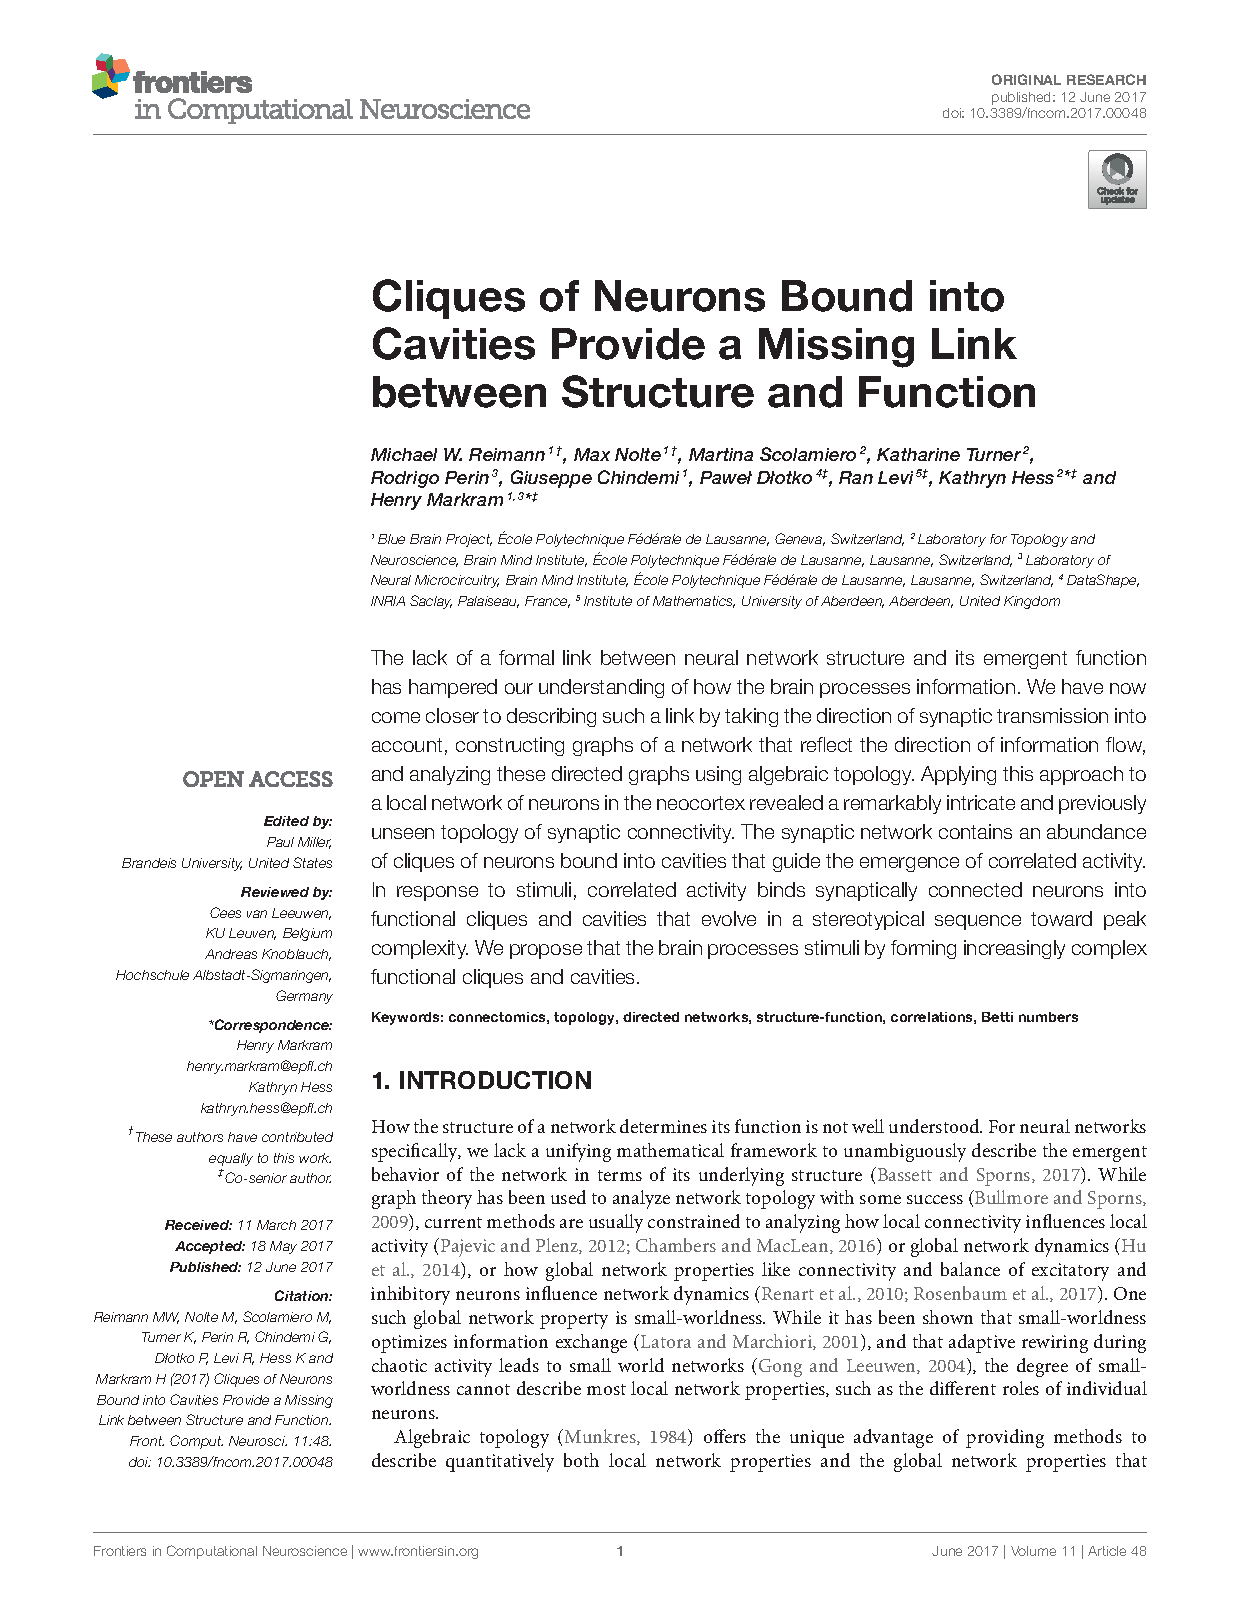
\includegraphics[height=5.2cm]{reimann.pdf}
\end{center}
\end{column}
\end{columns}
\end{frame}

\begin{frame}[label={sec:orga781094}]{Complejos simpliciales de gráficas dirigidas}
\begin{itemize}
\item En el artículo \emph{Cliques of Neurons Bound into Cavities Provide a Missing Link between Structure and Function} los autores forman una gráfica dirigida \(D\) donde los vértices son neuronas, y las flechas representan actividad neuronal.

\begin{center}
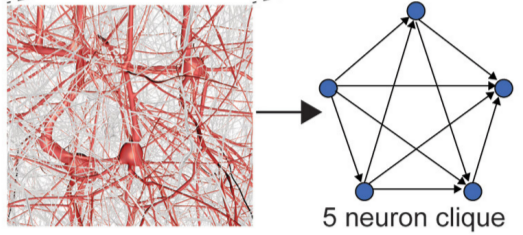
\includegraphics[width=7cm]{neuron.png}
\end{center}

\item Por simplicidad, supondremos que entre dos vértices dados de \(D\) existe cuando mucho una flecha.
\end{itemize}
\end{frame}

\begin{frame}[label={sec:org61708af}]{Simplejos}
\begin{itemize}
\item Los autores muestran que entre todos los torneos de \(n\) vértices, los que tienen mayor \emph{direccionalidad} son los acíclicos.

\bigskip

\begin{figure}[htbp]
\centering
\input{non-acyclic-acyclic.tikz}
\end{figure}
\end{itemize}

\pause\pause

\begin{itemize}
\item Los autores entonces le llaman \alert{clan dirigido} (\emph{directed clique}) a los \alert{torneos acíciclos}.

\item Como cualquier subgráfica de un torneo acíclico induce un torneo acíclico, podemos definir  un complejo simplicial \(\Delta(D)\) como el complejo simplicial cuyos simplejos son los subconjuntos de vértices de \(D\) que inducen torneos acíclicos.
\end{itemize}
\end{frame}

\begin{frame}[label={sec:org7ab3c63}]{Resultados}
Los autores estudiaron un modelo de una sección del cerebro de una rata. Y un modelo completo del gusano \emph{Caenorhabditis Elegans.} Una de sus conclusiones es:

\medskip

\begin{quote}
We found a remarkably high number and variety of high-dimensional directed cliques and cavities, which had not been seen before in neural networks, either biological or artificial, and in far greater numbers than those found in various null models of directed networks.
\end{quote}

\pause

\begin{center}
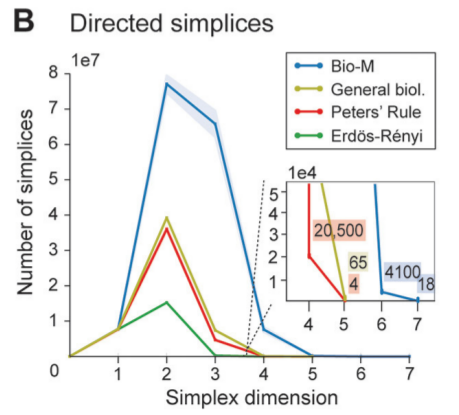
\includegraphics[height=3.5cm]{muchossimplejos.png}
\end{center}
\end{frame}

\begin{frame}
   \begin{center}
   \begin{huge}
   Gracias
   \end{huge}

  \bigskip
  \bigskip

  \begin{large}
  \faGithub{} \texttt{github.com/rvf0068/2021-coloquio-virtual}

   \bigskip

  \faTwitter{} \texttt{@rvf0068}

   \bigskip

   \faEnvelope{} \texttt{rafaelv@uaeh.edu.mx}

  \end{large}
  \end{center}
\end{frame}
\end{document}